\chapter{Analyse}

Das vorherige Kapitel beschrieb die nötigen Technologien für die Realisierung und Ausführung einer Anwendung im Microservice-Architektur-Stil.
Dieser Teil widmet sich mit den Innovationsforschungen der Krones AG in Form eines Proof of Concepts.
In diesem werden Technologien zur Modernisierung der Systemlandschaft untersucht, wie dem Edge-Computing und Kubernetes.


\section{Proof of Concept}\label{moderninfra}
Die Krones AG entwickelt neue Konzepte, um Produktionsanlagen standortübergreifend zu modernisieren. 
In einem davon wurde ein \ac{poc} mit dem Software-Unternehmen SUSE durchgeführt, um die Umsetzung neuer Cloud-Technologien zu evaluieren. 
Die folgenden Punkte behandeln die Kernthemen des \acs{poc} wie Edge-Computing und Kubernetes.

\subsection{Edge-Computing}
Edge-Computing bezeichnet die dezentrale Verarbeitung von Daten in direkter Nähe der Datenquelle. 
Das verringert den Bedarf an lokale Rechenzentren und senkt die Latenzzeiten bei der Übertragung von Daten. 
Betrachtungsgenstand des PoC war die Virtualisierung der bereits vorhandenen Industrierechner der Firma B\&R, um sie als Virtual-Edge-Devices zu verwenden.
Auf den Virtual-Edge-Devices werden dann Operationen wie erfassen, aggregieren und aufbereiten von Daten direkt an der Anlage ausgeführt. 
Die derzeitigen Anwendungen der Krones AG sind für das Betriebssystem Windows konzipiert und entwickelt worden.
Für das Edge-Szenario soll aber ein Linux basierte Betriebssystem verwendet werden,
weshalb die Integration über Virualisierungsmöglichkeiten realisiert wird.

\subsubsection{Virtualisierung}
Das Unternehmen B\&R steht in Kooperation mit der Firma RTS, diese bietet Technologie für die Virtualisierung von Echtzeit Betriebssystemen an \cite{rtosandbundr}.
Dafür wird ein Hypervisor genutzt, um gleichzeitig unterschiedliche Echtzeit Betriebssysteme in Form von VMs auszuführen.
Dies ermöglicht auch die Zuteilung von Hardwareressourcen auf den laufenden VMs.
Ein Vorteil ist das keine zusätzliche Hardware benötigt wird.
Die Zuweisung für Hardwareschnittstelen wie Ethernet USB-Ports ist durch diesen Ansatz auch möglich.
Virtuelle Netzwerke erlauben die Zuweisung von IPv4 und Mac-Adressen einzelner Prozessorkerne.
Diese ermöglichen eine direkte Kommunikation über Internetprotokolle wie TCP/IP oder COBRA.
Weiter kann jedes virtualisierte Betriebssystem Daten über einen gemeinsame Speicherpartitionen verwaltet werden \cite{rtos}.

\subsubsection{Connected \ac{hmi}}
Die Produktionsanlagen nutzen Windows 10 Embedded als Betriebssytem.
Darauf läuft das \acs{hmi} mit einer Touch-Oberfläche für Benutzereingaben.
Dies ist für die zentrale Überwachung und Steuerung von Analagenprozessen zuständig.
Und erlaubt die Einteilung von Produktionsrelevanten Aufgaben wie Wartungsarbeiten, Materialversorgung und Qualitätskontrollen \cite{hmi}.

\subsubsection{SUSE Linux Enterprise Micro}
Das für Edge-Szenarien entwickelte Open-Source-Betriebssystem SUSE Linux Enterprise Micro ist das zweite virtualisierte Betriebssystem, dass auf dem Hypervisor laufen soll.
Dieses arbeitet mit transactional-updates, welche Updates erst aktivieren, wenn das Betriebssystem neu gestartet wurde. 
Erfolgt das Update nicht wird ein Rollback zum vorherigen Versionszustand durchgeführt und ermöglicht wartungsfreie Zustände der Geräte.
Das Betriebssytem wurde, um die Idee von containerisierten Arbeistlasten und Microservices entwickelt.

\subsection{Kubernetes}
Auf der Grundlage des Edge-Computing war der zweite Schwerpunkt des PoC die Orchestrierung einer solchen Infrastruktur. 
Dabei sollen die einzelnen Virtual-Edge-Devices in Zukunft als Knotenpunkte für ein Kubernetes-Cluster dienen. 
Dafür wird die für Edge-Szenarien entworfene Kubernetes-Distribution k3s installiert.

Auf dieser sollen containerisierte Anwendungen ausgeliefert und bereitgestellt werden.
Anwendungen wie Mircoservices können innerhalb des Cluster über Endpunkte oder Kubernetes-Objekte kommunizieren.
Dadurch müssen Hostssysteme und der darauf laufenden Software nicht mit dessen Netzwerkadresse angesprochen werden.
Die Vorkonfiguration von Anwendung fällt durch die Architektur von Containern auch weg.



\subsubsection{Rancher}
Zur Orchestrierung der Kubernetes-Cluster Instanzen wurde die Orchestrierungsplattform Rancher näher untersucht. 
Diese ermöglicht die zentrale Verwaltung mehrerer Kubernetes-Cluster in Produktionsumgegebungen.
Weiterhin wurde die Bedienbarkeit der Benutzeroberfläche untersucht und es wurden Tests durchgeführt.
Bei diesen wurden containerisierte Arbeitslasten verwaltet und Kubernetes-Objekte erstellt und miteinander verbunden.
Ein weiterer Vorteil ist die Auslieferung von Kubernetes-Anwendungen durch den Apps \& Marketplace von Rancher. 

\subsubsection{Helm}
Helm ist ein Kubernetes-Package-Manager und ermöglicht die Erstellung, Installation und das Updaten von Kubernetes Anwendungen.
Wichtige Konzepte von Helm sind Charts, diese sind eine Ansammlung von Informationen zur Erstellung von Anwendungen als Kubernetes-Instanz. 
Config diese beinhalten die Informationen der Konfiguration von Charts und erstellen oder verpacken diese.
Release bezeichnet eine laufende Instanz eines Chart in Kombination einer bestimmten Config \cite{helm}.

Helm selber ist eine ausführbare Datei, die aus einem Kommandozeilentool besteht, dem Helm-Client.
Dieser erlaubt die lokale Entwicklung von Charts und dem verwalteten von Repositories wie auch der Versionsverwaltung.
Weiterhin dient der Client als Schnittstelle zur Helm-Library, welche Operationen mit dem Kubernetes-API-Server ermöglichen.
Dadurch können Charts und Konfigurationen als ein Release gebildet werden.
Weiterhin können Charts in einem Kubernetes-Cluster installiert werden.
Wie auch deinstalliert und aktualisiert werden. 
Die Konfigurationsdateien von Helm werden in der Regel, wie auch Kubernetes-Ressourcenobjekt in YAML geschrieben \cite{helm}.

Der Anwendungsfall im Bezug zur Krones AG ist die Kundenindividuelle Konfiguration von Kubernetes Anwendungen die in einem Kunden Repository gespeichert werden.
Die Kundenkonfigurationen stehen dabei als Helm-Charts verfügbar und ermöglichen eine vereinfachte Auslieferung und Bereitstellung durch Helm-Repositories.
Der Rancher Apps \& Marketplace ist hierbei eine Möglichkeit Helm-Charts, über eine Benutzeroberfläche zu konfigurieren und installieren.


\section{Anwendungsfälle}
Die Betrebungen des PoC zeigten neue Anwendungsfälle für die weitere Untersuchung des Kubernetes-Clusters.

\subsection{Hybrid Cloud}
Die zukünftige Kubernetes-Infrastruktur kann die Integration von On-Premise und Cloud-Ressourcen in einer Softwareumgegbung ermöglichen.



\subsection{Microservices}
\subsection{Künstliche Intelligenz}
\subsubsection{Deep Learning}



\section{Fachkonzept}
Im folgenden Abschnitt werden die Anforderungen und Anwendungsfälle für die spätere Konzeption der Microservice-Architektur erhoben.
Dafür wird ein zielorientierter Ansatz gewählt, der Anforderungen aus den Zielen einer Aufgabenstellung herleitet \cite[S.47]{Laplante}. 

\subsection{Anforderungserhebung}
Der vorherige Abschnitt \ref{moderninfra} beschreibt die Aufgabenstellungen, die mithilfe von Zielen erreicht werden können. 
Ziele sind erforderlich, um die zukünftigen Anforderungen der Software zu erarbeiten und werden in einer Anforderungstabelle wiedergeben (vgl. Tabelle~\ref{table:Anforderungstabelle}). 

\begin{table}[!htb]
\begin{center}

\begin{tabular}{|p{1cm}|p{6.8cm}|p{6.8cm}|l|l}
    \hline
    \textbf{Nr.} & \textbf{Ziele} & \textbf{Anforderungen} \\
    \hline
    \hypertarget{A01}{A01} 
    & Auf dem Kubernetes-Cluster laufen Anwendungen im Bereich der künstlichen Intelligenz.
    & Dienste sollen Funktionen der künstlichen Intelligenz ausführen können.
    \\
    \hline
    \hypertarget{A02}{A02}
    & Anwendungen auf einem Kubernetes-Cluster haben die Möglichkeit, Daten persistent zu speichern.
    & Dienste sollen über einen Speicher verfügen, der Daten persistent speichert.
    \\
    \hline
    \hypertarget{A03}{A03} 
    & Die einfache Auslieferung der Anwendung auf dem Kubernetes-Cluster ist möglich.
    & Die Dienste sollen über einen Auslieferungsmechanismus bereitgestellt werden.
    \\
    \hline
    \hypertarget{A04}{A04} 
    & Die Inbetriebnahme der Anwendung auf ein Kubernetes-Cluster ist vorkonfiguriert.
    & Dienste sollen vor der Inbetriebnahme vorkonfiguriert werden.
    \\
    \hline
    \hypertarget{A05}{A05} 
    & Die Anwendung funktioniert ohne die zusätzliche Installation von Abhängigkeiten auf dem Hostsystem.
    & Dienste sollen bei der Installation bereits über die nötigen Abhängigkeiten verfügen.
    \\
    \hline
    \hypertarget{A06}{A06} 
    & Die Anwendung kommuniziert in Echtzeit mit anderen Anwendungen auf dem Hostsystem.
    & Dienste sollen in Echtzeit miteinander kommunizieren.
    \\
    \hline
    \hypertarget{A07}{A07} 
    & Die Anwendung wurde vor der Inbetriebnahme auf dem Kubernetes-Cluster getestet.
    & Dienste sollen vor der Inbetriebnahme Tests durchlaufen.
    \\
    \hline
    \hypertarget{A08}{A08} 
    & Die Anwendung lässt sich für spezifische Hardware vorkonfigurieren. 
    & Dienste sollen bei Vorkonfiguration auf spezifischer Hardware laufen.
    \\
    \hline
\end{tabular}
\caption{Anforderungstabelle}
\label{table:Anforderungstabelle}
\end{center}
\end{table}

Die Tabelle gewährt einen groben Überblick der nötigen Systemanforderungen an die Mircoservice-Architektur. 
Diese werden nun im nächsten Abschnitt für das Konzept der Anwendung verwendet.
%Diese werden verfeinert und unterteilen sich im nächsten Abschnitt in Funktionale Anforderungen, also dem Grundverhalten, des Systems das der Nutzer erwartet und den nicht-Funktionale Anforderungen, den qualitativen oder leistungstechnischen Aspekten der Anwendung.



%\subsection{Funktionale Anforderungen}

%\textbf{Bereitstellung der Anwendung}: 
%Die Awendung muss sich auf einem Kubernetes Cluster, über eine Vorkonfiguration, bereitstellen lassen [\hyperlink{A01}{A01}]. 
%Bei der Bereitstellung muss die Anwendung, die nötigen Abhängigkeiten beeinhalten [\hyperlink{A05}{A05}]. 
%Zuletzt muss die Bereitstellung der Anwendung auf die Infrastruktur, Konfigurationen für spezifische Hardware enthalten [\hyperlink{A08}{A08}].
%Das 

%\textbf{Testprozess der Anwendung}: 
%Bevor die Anwendung verwendet wird, muss ein fester Testprozess die Funktionalität gewährleisten [\hyperlink{A07}{A07}].

%\textbf{Künstliche Intelligenz}: 
%Die Anwendung muss  [\hyperlink{A06}{A06}].



\subsection{Konzept}\label{Konzept}
Die prototypische Anwendung wird containerisiert und über eine Container-Registry verfügbar sein [\hyperlink{A03}{A03}] [\hyperlink{A05}{A05}]. 
Weiterhin muss die Anwendung unter der Berücksichtigung der Aspekte einer Microservice-Architektur, wie in Abschnitt \ref{Microservice} beschrieben, konzipiert und entwickelt werden. 
Die einzelnen Dienste der Anwendung müssen auf einem Kubernetes-fähigen Cluster ausgeliefert und in Betrieb genommen werden [\hyperlink{A04}{A04}].
Bevor die Anwendung verwendet wird, muss ein fester Testprozess die Funktionalität gewährleisten [\hyperlink{A07}{A07}].

Für die mögliche Auslieferung bei einem Kunden der Krones AG soll die Nutzung bereits vorhandener Hardware mit Grafikkarten möglich sein [\hyperlink{A08}{A08}]. 
Es ist vorgesehen, dass die Anwendung in einem hybriden Cloud-Szenario die vordefinierte Hardware nutzen kann. Folglich soll die Verwendung der Hardware zu einer verbesserten Leistungsauswertung von Modellen im Bereich der künstlichen Intelligenz führen. 
Arbeitslasten, wie dem Auswerten von Deep-Learning-Modellen wie im Falle der Linatronic AI \cite{linatronic}, sollen beispielhaft dargestellt werden [\hyperlink{A01}{A01}]. 
Dafür muss die Kommunikation von Diensten in Echtzeit stattfinden, um Informationen am Zielort schnell zu verarbeiten und eine nahtlose Verarbeitung großer Daten zu ermöglichen [\hyperlink{A06}{A06}].

\subsubsection{Anwendungsszenario}\label{Anwendungsszenario}

Der Schwerpunkt der zu entwickelnden Anwendung soll ein Dashboard mit Authentifizierungsmechanismus sein. 
Dieser soll Benutzern ermöglichen sich mit ihrem Passwort oder per Gesichtserkennung in ihr Profil einzuloggen. 
Die Daten sollen persistent gespeichert werden und können bei erneutem Aufruf der Website wieder verwendet werden [\hyperlink{A02}{A02}]. 

\subsection{Vorgehen}
Darauf aufbauend, wird im nächsten Schritt das fachliche Vorgehen zur Realisierung des Konzepts festgelegt.

\subsubsection{Komponententrennung von Diensten}
Wie in Abschnitt \ref{Microservice} behandelt werden die Kernfunktionalitäten der zu entwickelnden Anwendung  in einzelne Dienste aufgeteilt.
Im Systementwurf muss definiert werden über welche Schnittstellen die Dienste verfügen und über welche Endpunkte diese Erreichbar sind.
Folgend müssen auch die Service-Contracts zwischen den Diensten definiert werden.

\subsubsection{Auslieferungsstrategie}
Die Dienste müssen unabhängig voneinander auslieferbar sein.
Dienste verfügen über einem eigenen Speicherort, die aus dem Kubernetes-Cluster erreichbar ist.

\subsubsection{Bereitstellungsstrategie}
Bei der Bereistellung des Dienstes muss das Zielsystem über die notwendigen 

\subsubsection{Vorkonfiguration}


\section{Grobkonzeption}

Auf der Grundlage von Abschnitt \ref{Konzept} werden die Grobentwürfe erstellt.
Die Konzeptentwürfe gliedern sich in zwei Teile, der Infrastruktur und der Anwendung.

\subsection{Infrastruktur}
Die Abbildung \ref{fig:GrobentwurfInfrastruktur} stellt das Zielsystem dar.

\begin{figure}[!htb]
  \centering
  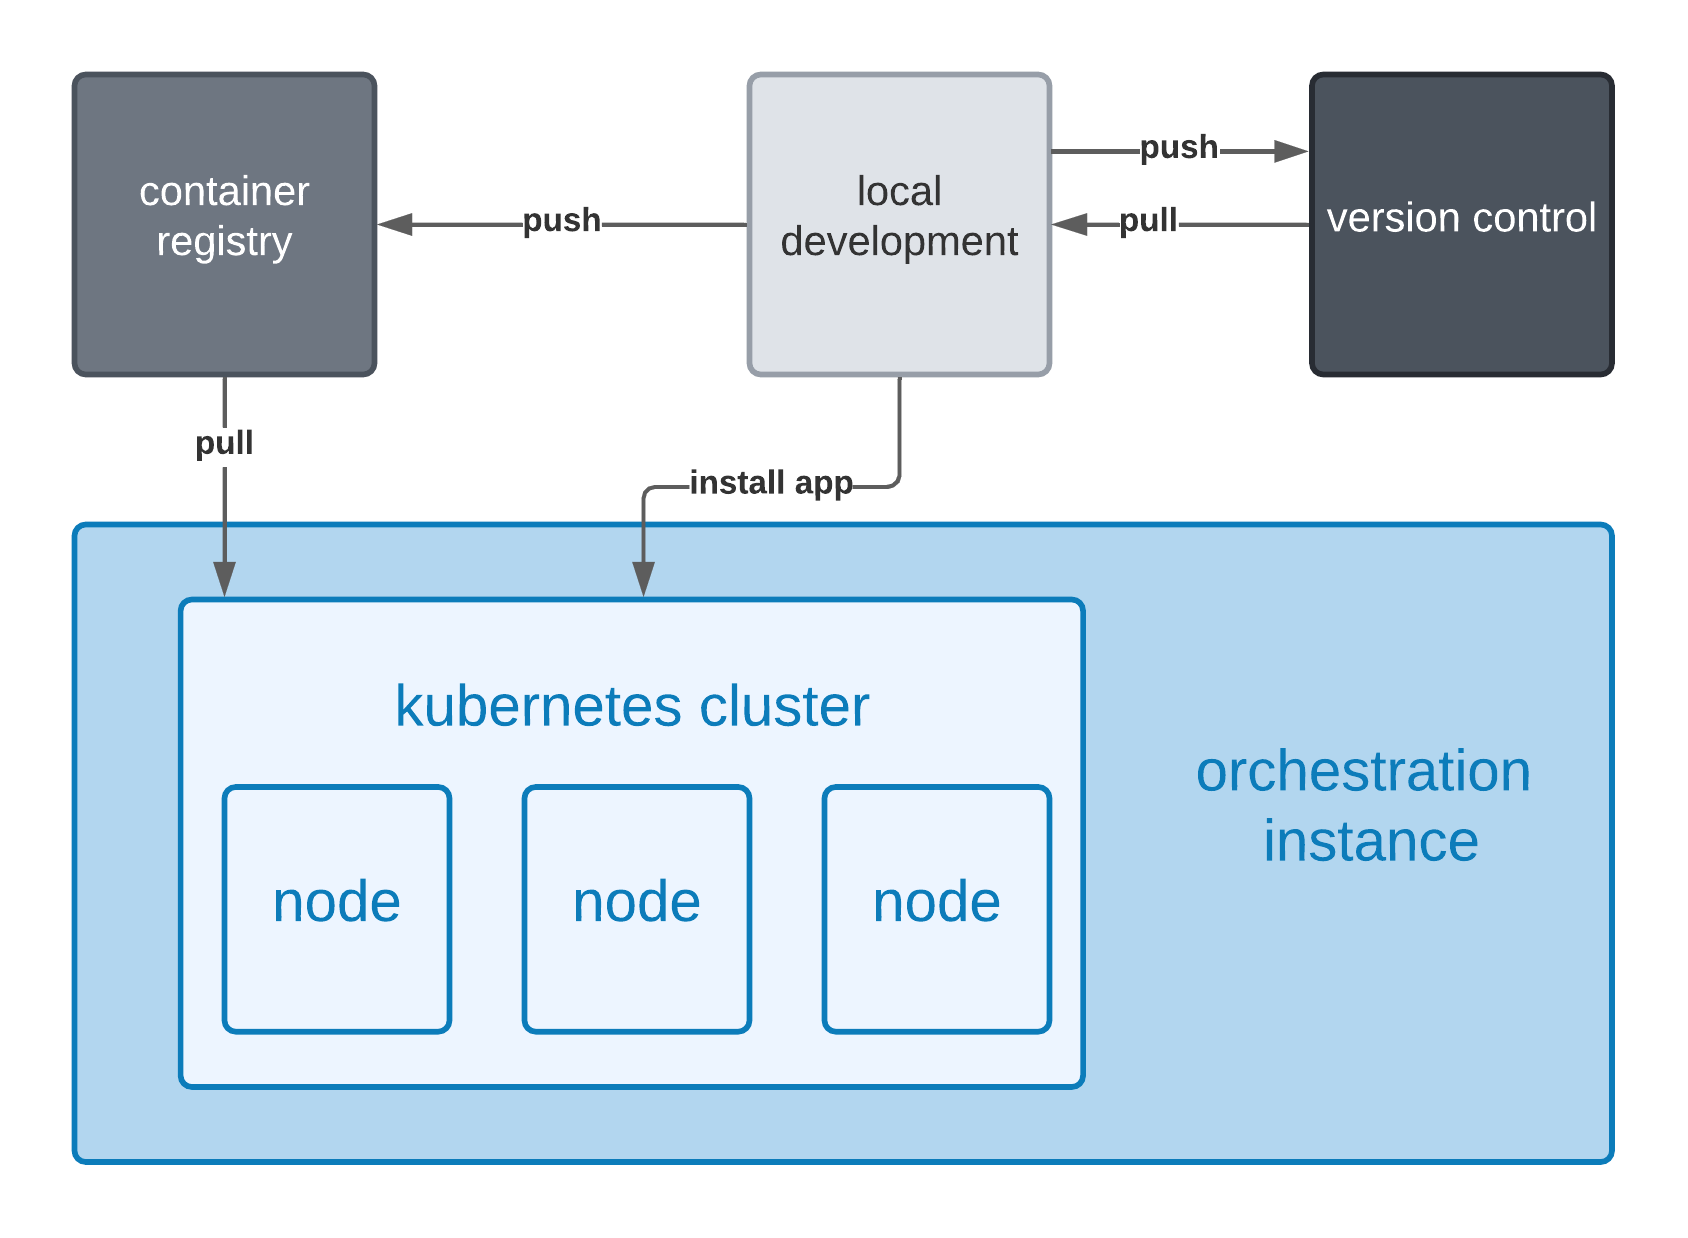
\includegraphics[width=0.8\columnwidth]{images/GrobentwurfInfrastruktur.png}
  \caption{Grobentwurf der Infrastruktur}
  \label{fig:GrobentwurfInfrastruktur}
\end{figure}

\textbf{Lokale Entwicklungsumgebung}: Die Entwicklung der Anwendung verläuft lokal und wird durch ein Versionsverwaltungssystem verwaltet.
Ein Befehl an das Kubernetes-Cluster initialisiert die Auslieferung und Bereitstellung der einzelnen Dienste. 

\textbf{Image-Registry}: Für die Auslieferung und Bereitstellung von Containern wird ein Image-Registry verwendet.
Dienste erhalten seperate Images und können unabhängig abgerufen werden.

\textbf{Kubernetes-Cluster}: Das Kubernetes-Cluster wird von einer Orchestierungsinstanz verwaltet.
Das Abrufen der Dienste erfolgt über ein Image-Registry.





\subsection{Anwendung}
Die Abbildung \ref{fig:GrobentwurfAnwendung} stellt das Anwendungszenario aus dem Unterabschnitt \ref{Anwendungsszenario} dar.
Die Anwendung aus dem Szenario wird in drei Dienste aufgeteilt.

\begin{figure}[!htb]
  \centering
  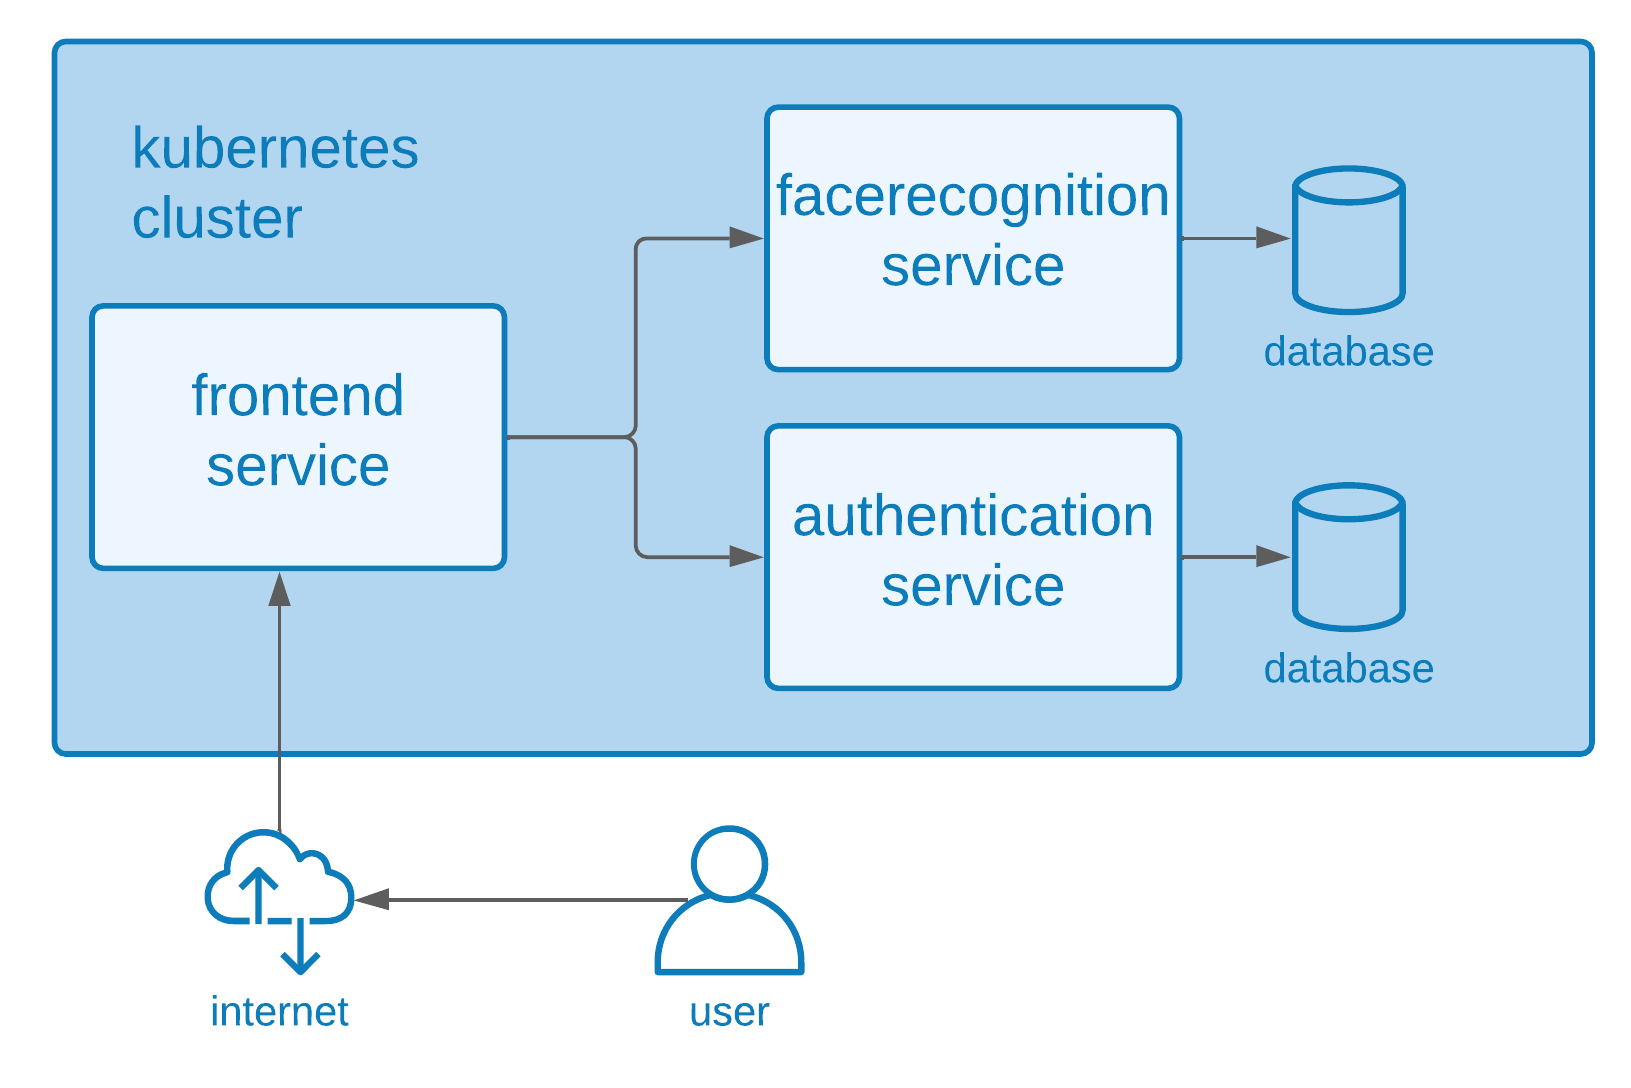
\includegraphics[width=0.8\columnwidth]{images/GrobentwurfAnwendung.png}
  \caption{Grobentwurf der Awendung}
  \label{fig:GrobentwurfAnwendung}
\end{figure}

\textbf{Frontend-Service}: Das Dashboard wird über den Frontend-Service bereitgestellt.
Darüber kann ein Benutzer die Funktionalitäten anderer Dienste nutzen.

\textbf{Authentication-Service}: Die Anmeldung und Registrierung in ein Nutzerkonto erfolgt über den Authentication-Service.
Dieser ermöglicht die persistente Speicherung der Nutzerdaten.

\textbf{Facedetection-Service}: Der Facedetection-Service bietet eine Anmeldung mithilfe von Gesichtserkennung an.
Die relevanten Daten zur Gesichtserkennung werden in einer Datenbank persistent gespeichert.

\subsection{Entwicklungsprozess}

Die Entwicklung der Anwendung wird in vier auf sich aufbauende Schichten eingeteilt (vgl. Abbildung~\ref{fig:Schichtenentwurf}).

\begin{figure}[!htb]
    \centering
    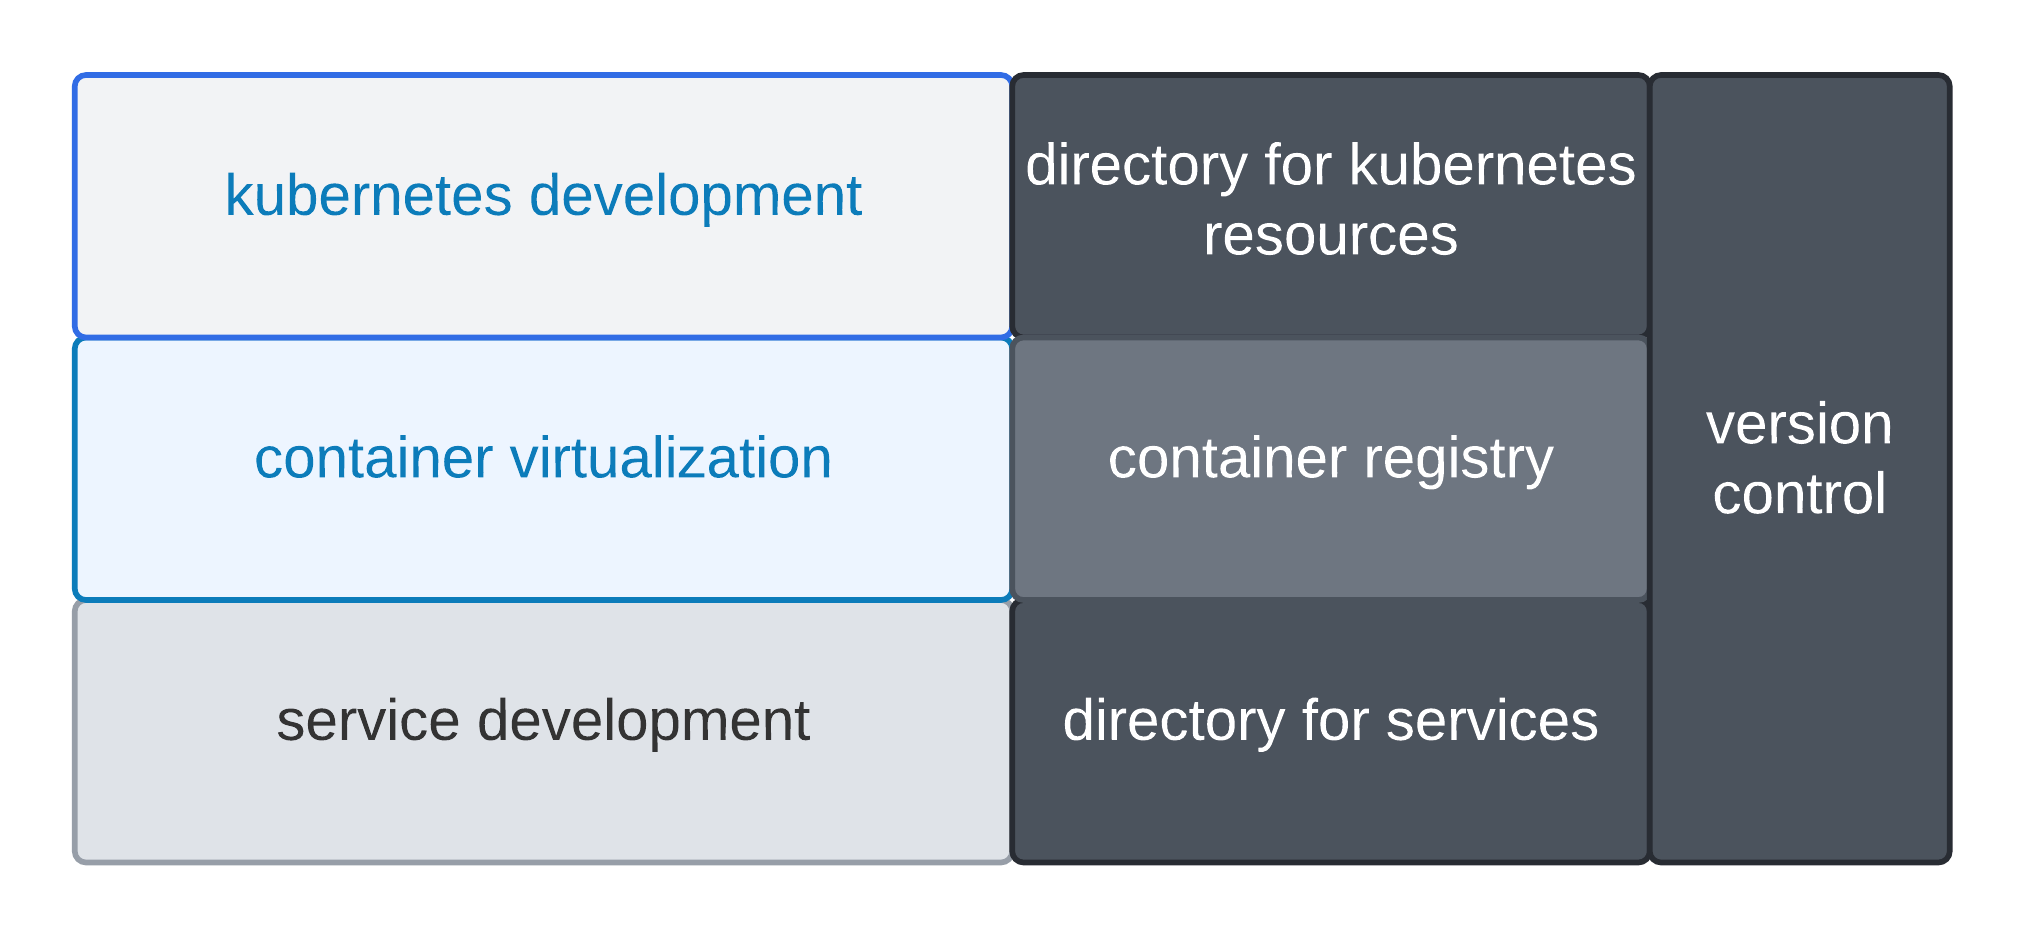
\includegraphics[width=1.0\columnwidth]{images/Schichtenentwurf.png}
    \caption{Vorgehen des Entwicklungsprozesses in Schichten}
    \label{fig:Schichtenentwurf}
  \end{figure}

\textbf{Anwendungsentwicklung}: 
Ein zentrales Repository beeinhaltet Verzeichnisse für die einzelnen Dienste.
Diese werden lokal entwickelt, getestet und ausgeführt.

\textbf{Containervirtualisierung}: 
Das entwickelte Programm wird dann containerisiert und weiterhin lokal ausgeführt.
Es wird getestet, ob die Containerisierung erfolgreich war und eine Kommmunikation untereinander möglich ist. 
Schließlich wird das Image auf ein öffentliches Registry hochgeladen. 
Jeder Dienst hat dabei einen eigenen Speicherort in Form eines Images.

\textbf{Kubernetes-Deployment}: 
Das zentrale Repository beinhaltet ein weiteres Verzeichnis für die Kubernetes-Ressourcenobjekte in Form von \acs{yaml}-Dateien.
Bei Zugang der Entwicklungsumgebung zu einem Kubernetes-Cluster können diese Dateien ausgeführt werden.

\textbf{Kubernetes-Cluster}: 
Das Testcluster wird aufgesetzt, installiert und in eine Orchestrierungsinstanz integriert.
Skripte für die Vorkonfiguration und Installation des Kubernetes-Clusters, erhalten ein eigenes Verzeichnis im zentralen Repository.
Die Auslieferung der Dienste erfolgt über das Image-Registry und werden von dem Kubernetes-Cluster heruntergeladen.



